% Created by tikzDevice version 0.12 on 2018-12-04 07:53:42
% !TEX encoding = UTF-8 Unicode
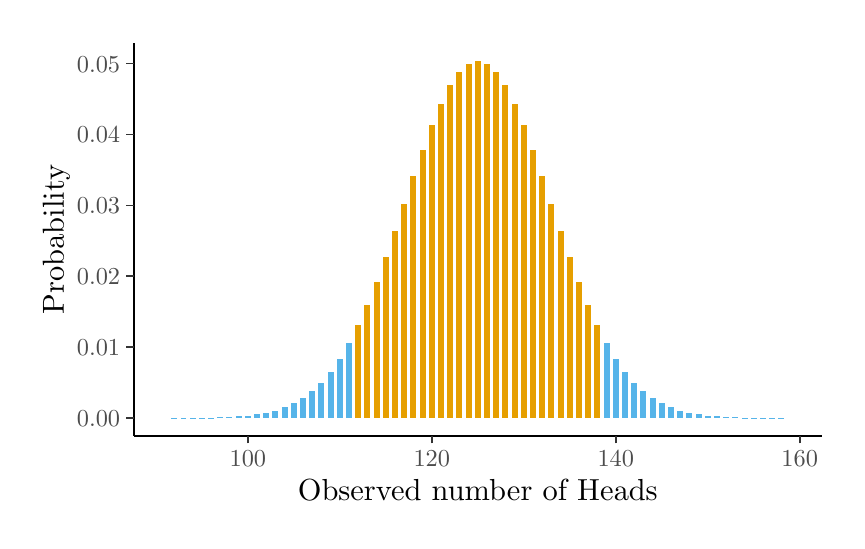
\begin{tikzpicture}[x=1pt,y=1pt]
\definecolor{fillColor}{RGB}{255,255,255}
\path[use as bounding box,fill=fillColor,fill opacity=0.00] (0,0) rectangle (292.45,178.21);
\begin{scope}
\path[clip] (  0.00,  0.00) rectangle (292.45,178.21);
\definecolor{drawColor}{RGB}{255,255,255}
\definecolor{fillColor}{RGB}{255,255,255}

\path[draw=drawColor,line width= 0.6pt,line join=round,line cap=round,fill=fillColor] (  0.00,  0.00) rectangle (292.45,178.21);
\end{scope}
\begin{scope}
\path[clip] ( 38.36, 30.72) rectangle (286.95,172.71);
\definecolor{fillColor}{RGB}{255,255,255}

\path[fill=fillColor] ( 38.36, 30.72) rectangle (286.95,172.71);
\definecolor{fillColor}{RGB}{86,180,233}

\path[fill=fillColor] ( 51.90, 37.18) rectangle ( 54.06, 37.20);

\path[fill=fillColor] ( 55.23, 37.18) rectangle ( 57.39, 37.21);

\path[fill=fillColor] ( 58.55, 37.18) rectangle ( 60.71, 37.23);

\path[fill=fillColor] ( 61.87, 37.18) rectangle ( 64.03, 37.27);

\path[fill=fillColor] ( 65.20, 37.18) rectangle ( 67.36, 37.33);

\path[fill=fillColor] ( 68.52, 37.18) rectangle ( 70.68, 37.42);

\path[fill=fillColor] ( 71.84, 37.18) rectangle ( 74.00, 37.55);

\path[fill=fillColor] ( 75.17, 37.18) rectangle ( 77.33, 37.75);

\path[fill=fillColor] ( 78.49, 37.18) rectangle ( 80.65, 38.04);

\path[fill=fillColor] ( 81.81, 37.18) rectangle ( 83.97, 38.45);

\path[fill=fillColor] ( 85.14, 37.18) rectangle ( 87.30, 39.04);

\path[fill=fillColor] ( 88.46, 37.18) rectangle ( 90.62, 39.85);

\path[fill=fillColor] ( 91.78, 37.18) rectangle ( 93.94, 40.96);

\path[fill=fillColor] ( 95.11, 37.18) rectangle ( 97.27, 42.44);

\path[fill=fillColor] ( 98.43, 37.18) rectangle (100.59, 44.37);

\path[fill=fillColor] (101.75, 37.18) rectangle (103.91, 46.86);

\path[fill=fillColor] (105.08, 37.18) rectangle (107.24, 49.99);

\path[fill=fillColor] (108.40, 37.18) rectangle (110.56, 53.87);

\path[fill=fillColor] (111.72, 37.18) rectangle (113.88, 58.58);

\path[fill=fillColor] (115.05, 37.18) rectangle (117.21, 64.17);
\definecolor{fillColor}{RGB}{230,159,0}

\path[fill=fillColor] (118.37, 37.18) rectangle (120.53, 70.67);

\path[fill=fillColor] (121.69, 37.18) rectangle (123.85, 78.08);

\path[fill=fillColor] (125.02, 37.18) rectangle (127.18, 86.34);

\path[fill=fillColor] (128.34, 37.18) rectangle (130.50, 95.31);

\path[fill=fillColor] (131.66, 37.18) rectangle (133.82,104.84);

\path[fill=fillColor] (134.99, 37.18) rectangle (137.15,114.67);

\path[fill=fillColor] (138.31, 37.18) rectangle (140.47,124.52);

\path[fill=fillColor] (141.63, 37.18) rectangle (143.79,134.06);

\path[fill=fillColor] (144.96, 37.18) rectangle (147.12,142.94);

\path[fill=fillColor] (148.28, 37.18) rectangle (150.44,150.80);

\path[fill=fillColor] (151.60, 37.18) rectangle (153.76,157.32);

\path[fill=fillColor] (154.93, 37.18) rectangle (157.09,162.21);

\path[fill=fillColor] (158.25, 37.18) rectangle (160.41,165.23);

\path[fill=fillColor] (161.57, 37.18) rectangle (163.73,166.26);

\path[fill=fillColor] (164.90, 37.18) rectangle (167.06,165.23);

\path[fill=fillColor] (168.22, 37.18) rectangle (170.38,162.21);

\path[fill=fillColor] (171.54, 37.18) rectangle (173.70,157.32);

\path[fill=fillColor] (174.87, 37.18) rectangle (177.03,150.80);

\path[fill=fillColor] (178.19, 37.18) rectangle (180.35,142.94);

\path[fill=fillColor] (181.51, 37.18) rectangle (183.68,134.06);

\path[fill=fillColor] (184.84, 37.18) rectangle (187.00,124.52);

\path[fill=fillColor] (188.16, 37.18) rectangle (190.32,114.67);

\path[fill=fillColor] (191.49, 37.18) rectangle (193.65,104.84);

\path[fill=fillColor] (194.81, 37.18) rectangle (196.97, 95.31);

\path[fill=fillColor] (198.13, 37.18) rectangle (200.29, 86.34);

\path[fill=fillColor] (201.46, 37.18) rectangle (203.62, 78.08);

\path[fill=fillColor] (204.78, 37.18) rectangle (206.94, 70.67);
\definecolor{fillColor}{RGB}{86,180,233}

\path[fill=fillColor] (208.10, 37.18) rectangle (210.26, 64.17);

\path[fill=fillColor] (211.43, 37.18) rectangle (213.59, 58.58);

\path[fill=fillColor] (214.75, 37.18) rectangle (216.91, 53.87);

\path[fill=fillColor] (218.07, 37.18) rectangle (220.23, 49.99);

\path[fill=fillColor] (221.40, 37.18) rectangle (223.56, 46.86);

\path[fill=fillColor] (224.72, 37.18) rectangle (226.88, 44.37);

\path[fill=fillColor] (228.04, 37.18) rectangle (230.20, 42.44);

\path[fill=fillColor] (231.37, 37.18) rectangle (233.53, 40.96);

\path[fill=fillColor] (234.69, 37.18) rectangle (236.85, 39.85);

\path[fill=fillColor] (238.01, 37.18) rectangle (240.17, 39.04);

\path[fill=fillColor] (241.34, 37.18) rectangle (243.50, 38.45);

\path[fill=fillColor] (244.66, 37.18) rectangle (246.82, 38.04);

\path[fill=fillColor] (247.98, 37.18) rectangle (250.14, 37.75);

\path[fill=fillColor] (251.31, 37.18) rectangle (253.47, 37.55);

\path[fill=fillColor] (254.63, 37.18) rectangle (256.79, 37.42);

\path[fill=fillColor] (257.95, 37.18) rectangle (260.11, 37.33);

\path[fill=fillColor] (261.28, 37.18) rectangle (263.44, 37.27);

\path[fill=fillColor] (264.60, 37.18) rectangle (266.76, 37.23);

\path[fill=fillColor] (267.92, 37.18) rectangle (270.08, 37.21);

\path[fill=fillColor] (271.25, 37.18) rectangle (273.41, 37.20);
\end{scope}
\begin{scope}
\path[clip] (  0.00,  0.00) rectangle (292.45,178.21);
\definecolor{drawColor}{RGB}{0,0,0}

\path[draw=drawColor,line width= 0.6pt,line join=round] ( 38.36, 30.72) --
	( 38.36,172.71);
\end{scope}
\begin{scope}
\path[clip] (  0.00,  0.00) rectangle (292.45,178.21);
\definecolor{drawColor}{gray}{0.30}

\node[text=drawColor,anchor=base east,inner sep=0pt, outer sep=0pt, scale=  0.88] at ( 33.41, 34.15) {0.00};

\node[text=drawColor,anchor=base east,inner sep=0pt, outer sep=0pt, scale=  0.88] at ( 33.41, 59.75) {0.01};

\node[text=drawColor,anchor=base east,inner sep=0pt, outer sep=0pt, scale=  0.88] at ( 33.41, 85.36) {0.02};

\node[text=drawColor,anchor=base east,inner sep=0pt, outer sep=0pt, scale=  0.88] at ( 33.41,110.96) {0.03};

\node[text=drawColor,anchor=base east,inner sep=0pt, outer sep=0pt, scale=  0.88] at ( 33.41,136.57) {0.04};

\node[text=drawColor,anchor=base east,inner sep=0pt, outer sep=0pt, scale=  0.88] at ( 33.41,162.17) {0.05};
\end{scope}
\begin{scope}
\path[clip] (  0.00,  0.00) rectangle (292.45,178.21);
\definecolor{drawColor}{gray}{0.20}

\path[draw=drawColor,line width= 0.6pt,line join=round] ( 35.61, 37.18) --
	( 38.36, 37.18);

\path[draw=drawColor,line width= 0.6pt,line join=round] ( 35.61, 62.78) --
	( 38.36, 62.78);

\path[draw=drawColor,line width= 0.6pt,line join=round] ( 35.61, 88.39) --
	( 38.36, 88.39);

\path[draw=drawColor,line width= 0.6pt,line join=round] ( 35.61,113.99) --
	( 38.36,113.99);

\path[draw=drawColor,line width= 0.6pt,line join=round] ( 35.61,139.60) --
	( 38.36,139.60);

\path[draw=drawColor,line width= 0.6pt,line join=round] ( 35.61,165.20) --
	( 38.36,165.20);
\end{scope}
\begin{scope}
\path[clip] (  0.00,  0.00) rectangle (292.45,178.21);
\definecolor{drawColor}{RGB}{0,0,0}

\path[draw=drawColor,line width= 0.6pt,line join=round] ( 38.36, 30.72) --
	(286.95, 30.72);
\end{scope}
\begin{scope}
\path[clip] (  0.00,  0.00) rectangle (292.45,178.21);
\definecolor{drawColor}{gray}{0.20}

\path[draw=drawColor,line width= 0.6pt,line join=round] ( 79.57, 27.97) --
	( 79.57, 30.72);

\path[draw=drawColor,line width= 0.6pt,line join=round] (146.04, 27.97) --
	(146.04, 30.72);

\path[draw=drawColor,line width= 0.6pt,line join=round] (212.51, 27.97) --
	(212.51, 30.72);

\path[draw=drawColor,line width= 0.6pt,line join=round] (278.97, 27.97) --
	(278.97, 30.72);
\end{scope}
\begin{scope}
\path[clip] (  0.00,  0.00) rectangle (292.45,178.21);
\definecolor{drawColor}{gray}{0.30}

\node[text=drawColor,anchor=base,inner sep=0pt, outer sep=0pt, scale=  0.88] at ( 79.57, 19.71) {100};

\node[text=drawColor,anchor=base,inner sep=0pt, outer sep=0pt, scale=  0.88] at (146.04, 19.71) {120};

\node[text=drawColor,anchor=base,inner sep=0pt, outer sep=0pt, scale=  0.88] at (212.51, 19.71) {140};

\node[text=drawColor,anchor=base,inner sep=0pt, outer sep=0pt, scale=  0.88] at (278.97, 19.71) {160};
\end{scope}
\begin{scope}
\path[clip] (  0.00,  0.00) rectangle (292.45,178.21);
\definecolor{drawColor}{RGB}{0,0,0}

\node[text=drawColor,anchor=base,inner sep=0pt, outer sep=0pt, scale=  1.10] at (162.65,  7.44) {Observed number of Heads};
\end{scope}
\begin{scope}
\path[clip] (  0.00,  0.00) rectangle (292.45,178.21);
\definecolor{drawColor}{RGB}{0,0,0}

\node[text=drawColor,rotate= 90.00,anchor=base,inner sep=0pt, outer sep=0pt, scale=  1.10] at ( 13.08,101.72) {Probability};
\end{scope}
\end{tikzpicture}
